\documentclass[12pt,a4paper]{report}
\usepackage[utf8]{inputenc}
\usepackage{amsmath}
\usepackage{amsfonts}
\usepackage{amssymb}
\usepackage{makeidx}
\usepackage{comment}
\usepackage{graphicx}
\usepackage{lmodern}
\usepackage{forest}
\usepackage{fixltx2e}
\usepackage{kpfonts}
\usepackage{listings}
\usepackage{rotating}
\usepackage{listings-golang} % import this package after listings
\usepackage[left=3.5cm,right=2.5cm,top=2.5cm,bottom=3cm]{geometry}
\author{Nikolas Pafitis\\\\\\ Supervisor\\Chryssis Georgiou}
\date{May 2019}
\renewcommand{\baselinestretch}{1.5}
\title{University Of Cyprus \\ \smaller{Computer Science Department} \\
Implementation of Self-Stabilizing BFT using Go and ZeroMQ}
\pagenumbering{roman}

\lstset{ % add your own preferences
    frame=single,
    basicstyle=\footnotesize,
    keywordstyle=\color{red},
    numbers=left,
    numbersep=4pt,
    showstringspaces=false, 
    stringstyle=\color{blue},
    tabsize=4,
    language=Golang % this is it !
}

\begin{document}
\begin{titlepage}
	\centering
	\begin{comment}
	\includegraphics[width=0.15\textwidth]{example-image-1x1}\par\vspace{1cm}
	\end{comment}
	{\scshape\LARGE University Of Cyprus \par}
	\begin{comment}
	\vspace{1cm}
	\end{comment}
	{\scshape\Large Department of Computer Science\par}
	\vfill
	{\Large\bfseries Implementation of Self-Stabilizing BFT Using Go and ZeroMQ\par}
	\vspace{1cm}
	{\Large\bfseries Nikolas Pafitis\par}
	\vfill
	Supervisor\par
	Chryssis Georgiou

	\vfill
	
	The Individual Diploma Thesis was submitted for partial fulfillment of the requirements of obtaining the degree of Computer Science of the Department of Computer Science of the University of Cyprus
	
	\vfill

% Bottom of the page
	{\large {May 2019}\par}
\end{titlepage}
\thispagestyle{empty}



	\abstract{Byzantine Fault Tolerant algorithms have been under research for many years as they provide systems protection against failures and malicious attacks. This thesis presents an implementation\cite{implementation} in the Go programming language of the first self-stabilizing BFT algorithm by S. Dolev, C. Georgiou, I. Marcoullis and E. Schiller \cite{ssbft} to investigate the applicability of the algorithm in Go, and the algorithm's functionality in real-world-like applications. After experimental assessment, we conclude that our self-stabilizing version is only 8\% slower than its non-self-stabilizing counterpart, and that the time that it takes to converge from a state with stale information is practically equal to six to seven times the time that it takes for the system to serve a request, and the convergence time for a system with a byzantine primary is approximately equal to ten times the average serve time.
}
	
% 	\addtocontents{toc}{\protect\setcounter{tocdepth}{-1}}
    \setcounter{secnumdepth}{3}
    \setcounter{tocdepth}{3}
	\tableofcontents
	



	
	\chapter{Introduction}
	\pagenumbering{arabic}

	\setcounter{page}{1}
		\section{Incentive}
			In modern times, cloud computing or cloud systems are terms used to describe the computer elements, either that be software, hardware or 
				infrastructure, that can provide computer services that come in various forms such as Platform as a Service (PaaS), Software as a Service (SaaS)
				and Infrastructure as a Service (IaaS), to users and corporations over the Internet, either that service is storing consumers' data or some
				sort of computation. That means that a lot of other services and applications
				are critically dependent on the correct operation of such systems.
				Thus, continuous operation of cloud systems is absolutely necessary, otherwise the consequences are so severe that the use of cloud systems
				is rendered useless.

		
			Key issues of cloud systems are reliability, meaning that data stored is never lost and that services provided are always correct and
				available, security, as cloud systems are currently one of the main targets of malicious attacks, performance, since otherwise the value of
				using cloud products is nullified, scalability so that it is able to support consumers regardless of any sudden change in the amount of users
				consuming said service while maintaining same levels of performance. That said, the challenge confronted in maintaining
				cloud computing services is tremendously difficult for systems that are going to serve 
				millions globally and even more so when said systems are distributed globally.   
	
			
			So providers of cloud computing services to facilitate the difficulty that maintaining these kinds of services imply, make up for it by
			utilizing redundant amount of processors and replicating over those processors in case a processor fails, to operate	these services and/or 
			to store the data of its consumers, making this practice excessively expensive. Thus, the need for fast fault tolerant algorithms emerges.
			

				One such solution is the algorithm implemented in a paper by S. Dolev, C. Georgiou, I. Marcoullis and E. Schiller\cite{ssbft} which is an enhanced version of Castro and Liskov's Practical Byzantine Fault Tolerance (PBFT) \cite{pbft} that also deploys the
				property of Self-Stabilization. It uses State Machine Replication (SMR) based on Failure Detectors,
				to implement fault-tolerance and replica consistency, imposing an
				ordering of state transitions to replicas of correct processors. BFT grants the ability to replicate even in the presence of Byzantine
				processors, although it implies a series 
				of assumptions. Most BFT implementations assume that the initial state of processors' replicas is consistent among processors. Other assume 
				that the initial system variables are consistent among processors. Liveness assumptions are also required, meaning some kind of
				synchronization of sorts and/or failure detection and others. Even though a BFT system will behave as intended even if some of its processors
				are malicious or experience Byzantine faults, it is necessary for a human system administrator to recover compromised processors. On the other 
				hand  self-stabilizing systems are able to recover automatically from any behaviour temporarily deviating from its specification without the need of a system administrator. Thus 
				shaping self-stabilizing algorithms to be quite valuable in distributed and cloud applications.
		\section{Objective}
			    Objective of this work is to implement the self-stabilizing Byzantine Fault Tolerant State Machine Replication algorithm\cite{ssbft},
				executing it in real-world-like simulations, validate whether the algorithm's purpose is achieved, and comparing its performance against Castro and Liskov's classic example, and survey its
				applicability in real applications, by taking numerous measures such as time needed to converge to a legal state, overhead of self-stability
				in terms of average request serve time and determine the difficulty of implementing it.
		\section{Implementation}
			For this implementation we'll use the Go (or Golang) as the programming language and the ZeroMQ (ZeroMQ or 0MQ) messaging library as the mean of
				communication
				between	nodes.  Using the Go programming language comes with several benefits and compromises. It is a statically-types language, meaning that
				our implementation will be less prone to mistype errors. It is also compiled, has structural typing similar to C, and provides form of Object-Oriented programming that is exclusive to Go, but very useful nonetheless. Though most notably, it comes with built-in framework for
				concurrency in the form of Goroutines (fancy name for co-routines), over the Communicating sequential processes (CSP) concurrency paradigm. 
				Goroutines are green-threads that are as easy to spawn as just adding a dedicated keyword before a procedure call (i.e go callFunc()).
				Similarly the ZeroMQ library is the perfect fit for this project as it is a incredibly high-performance asynchronous messaging queue that
				runs without a dedicated message broker. Messages sent through ZeroMQ are guaranteed to reach their destination and it provides numerous of
				messaging patterns and socket
				types for every type of topology and architecture through a very usable Application Programming Interface (API).
		\section{Methodology}
		
			\subsection{Research on Distributed Systems}
			For the realization of my undergraduate thesis I went through studying the literature regarding Distributed
			Systems, Byzantine Fault-Tolerance, Self-Stabilization and ZeroMQ. In terms of Distributed Systems I studied the lecture notes of the
			Graduate's Computer Science course, EPL601 Distributed Systems, solved various examples, exercises and projects about process management,
			signals, low-level input/output, forking processes and process communication in C programming language that were part of the course. I also
			studied the article "A brief introduction to distributed systems" by Maarten Van Steen and Andrew S. Tanenbaum (2016) \cite{distributedSystems}
			to acquire a brief overview of Distributed Systems, their general design goals and common types of architectures of Distributed Systems.
			I've also learned how distributed systems are a collection of autonomous computing elements and that a distributed system should appear to
			the user as a single coherent system, meaning that information about each particular node should be hidden by the end-user, otherwise known as
			\textbf{distribution transparency}.

			
			\subsection{Research on BFT}
				With respect to Byzantine Fault-Tolerance, I examined the original article of Castro and Liskov, Practical Byzantine Fault Tolerance
				\cite{pbft}, the first description of a replication algorithm that is able to tolerate Byzantine faults, preventing faulty nodes to exhibit
				arbitrary behaviour. It describes an algorithm where it more or less functions as follows
				\begin{itemize}
				    \item A group of processors serve a group of clients by replicating the clients' requests.
				    \item At any given time, exactly one processor is assigned to be the primary processor.
					\item A client requests a service operation by sending a message to the primary
					\item Primary broadcasts the client's request to the rest of the processors
					\item Processors then execute the request and reply to the client with the result
					\item Client waits for f + 1 replies with the same result, where f is the allowed amount of faulty processors.
				\end{itemize}
				

			
			\subsection{Research on Self-Stabilization}
			In regards to Self-Stabilization, I've read the paper "Self-Stabilization" by Marco Schneider\cite{ss} and acquired knowledge about the notion of
			self-stabilizing systems, the definition of Self-Stabilization, the meaning of closure and convergence to a legal state, its history and about
			self-stabilization in general as an approach to fault tolerance. Next, I thoroughly went through the paper describing the self-stabilizing BFT by S. Dolev, C. Georgiou, I. Marcoullis and E. Schiller \cite{ssbft}, went through the details of
			the	algorithm and I compared it	against Castro and Liskov's version to get a broader view of the self-stabilizing version and how it is modified
			for the original, and to get a better understanding of the internals of the algorithm.

			
			\subsection{ZeroMQ}
			As far as ZeroMQ goes, I've studied upon ZeroMQ's reference manual\cite{zmqref} to get grasp of the available programming interface, and later
			the ZeroMQ's ZGuide\cite{zguide}, learning all about the different kinds of socket types and messaging patterns and architecture that ZeroMQ
			provides. While reading the ZGuide I have implemented all of it's programming examples and patterns both in C and Go programming languages, 
			while also referring to the online Git Hub repository\cite{zguidegit} with implementations of the book's examples in over 30 different programming
			languages.


			\subsection{Development}
    			As I was developing the system, I tested it locally on my personal computer for debugging and validating correct operation of the algorithm. After I made sure that all operations are as intended evaluated it's performance and behaviour in real-world environment at the PlanetLab Europe \cite{planetLab} in a slice allocated to me by my supervisor. PlanetLab is a planetary scale networked system that is used as a testbed for the development and research of computer networks and distributed systems in a reliable experimental environment. I tested it over different scenarios, like initializing the system in non-consistent states, having faulty-processors, having a Byzantine primary processor, and comparing it's operation against that of Castro and Liskov's version while examining the overhead costs of Self-Stabilization.
    			
    	\section{Document Organization}
    	    In Chapter 2 we make a background retrospective on Byzantine Failure and Byzantine Fault Tolerance, the Self-Stabilization property of systems, ZeroMQ messaging library, and the Go programming language. In Chapter 3 we give a thorough explanation of the self-stabilizing BFT algorithm and we provide a detailed description of our implementation and the factors behind our decisions. Next, in Chapter 4 we portray our experimental environment (PlanetLab\cite{planetLab}) and our experimental scenarios which we designed to confirm the functionality of our implementation, and we discuss the results that we achieved.
				
	\newpage

	\chapter{Background}
		\section{Byzantine Failure}
			\subsection{Byzantine Faults}
			Byzantine Faults or Failures is a term used to describe a computer system condition, more commonly used in distributed computing systems, where 
			components comprising the system can be faulty and information about their faultiness is incomplete\cite{bf}. The term's name stems from an
			the "Byzantine Generals Problem"\cite{generals} thought experiment where it describes a situation of a group of generals communicating only by 
			messenger that have to agree upon a common battle plan, but one or more traitors will try and confuse the rest. The usual correlation of this allegory in terms computer systems is that computers are the generals and the links of the digital communication systems are the messengers. Although the problem is expressed in analogy as a decision-making and security problem in electronics, it can not be solved simply by cryptographic digital signatures, because failures such as incorrect voltage can be propagated through the encryption process. Therefore, a component may look functional to one component and defective to another, which prevents consensus formation if the element is defective or not.
			

			 Another definition of a Byzantine
			Fault is that a Byzantine fault is any fault presenting different symptoms to different observers\cite{realgenerals}. Byzantine failures are
			considered to be the most general and most difficult category of failure. Byzantine failures do not imply any constraints, which means that the
			failed node can produce arbitrary data pretending it is correct. Thus,
			Byzantine failures can cause confusion in fault detection systems, making tolerance to error difficult. Despite the analogy, a Byzantine failure
			is not necessarily a security problem involving hostile human intervention: it can only arise from electrical faults.

			\subsection{Byzantine Fault Tolerance}
			Like in the anecdote of the	blind men feeling an elephant and making assumptions about what's the elephant's shape, in Byzantine Fault tolerant
			systems, processors have to come to a consensus about whether some processor is faulty or not even if some of them are byzantine. In general, 
			Byzantine fault tolerance mechanisms use elements that repeat an incoming message to other recipients of the same incoming message. All these
			mechanisms make the assumption that the act of repeating a message prevents the spread of Byzantine symptoms.
			For systems that have a high degree of safety or security criticality, these assumptions must prove valid at an acceptable level of error
			coverage. When we offer proof through the tests, a difficulty creates a sufficiently wide range of signals with Byzantine symptoms. These
			tests may require specialized spray injectors.
			The objective of Byzantine fault tolerance is to be able to defend against failures of system components with or without symptoms that prevent
			other components of the system from reaching an agreement among themselves, where such an agreement is needed for the correct operation of the
			system. Early solutions can be traced as far back as 1982 by Lamport, Shostak, and Pease\cite{generals} where they noted that a Byzantine Generals
			 problem can
			be reduced to a "Commander and Lieutenants" problem where loyal lieutenants must all act together and their action responds to what the commander
			has ordered under the assumption that the commander is loyal. Miguel Castro and Barbara Liskov in 1999\cite{pbft}, introduced the Practical
			Byzantine Fault Tolerance algorithm, which describes a high-performance solution to the Byzantine Generals problem, implementing a Byzantine fault
			tolerant NFS system with only a 3\% latency than a standard unreplicated NFS service. After PBFT, many variations of it where introduced to 
			improve robustness and performance such as  Q/U\cite{qu}, Zyzzyva\cite{zyzzyva} and ABsTRACTs\cite{abstracts}.

			\subsection{Common Applications of BFT}
			Common applications of BFT can be found in distributed cloud computing systems, networked file systems, but also in some aircraft systems such as
			Boeing 777's Aircraft Information Management System and flight control system and SpaceX's Dragon spacecraft flight systems since these are
			examples of real-time systems and require very low latency solutions. Most notably, an example of the BFT is used in Bitcoin, a peer-to-peer 
			system implementing digital currency. The Bitcoin network works in parallel to create a blockchain with proof of work that allows the system to 
			overcome Byzantine failures and reach a comprehensive overall view of the state of the system.
			
		\section{Self-Stabilization}
			\subsection{Definition of Self-Stabilization}
			Self-stabilization comes with two properties, convergence and closure. A system is self-stabilizing if and only if it satisfies the following \cite{dolev}:
			\begin{itemize}
					\item Convergence: No matter whether the initial state is legal or not, the system is guaranteed that it will eventually reach a legal state.
					\item Closure: Given that a system is found in a legal state, the system is guaranteed to stay in a legal state, as long as no further transient fault 
					happens.
					\item A state is legal if starting from this state the algorithm satisfies its         specification.
			\end{itemize}
			

			The ability to self-stabilize allows a distributed algorithm to recover from a transient fault, regardless of its nature. Moreover, there is no 
			need to initialize a self-stabilization algorithm, as it eventually begins to behave properly regardless of its original state. The first self-
			stabilizing algorithms did not explicitly detect errors in order to fix them later. Instead, they constantly made the system a legal situation. 
			Since traditional error detection methods were often very difficult and time-consuming, such behavior was considered desirable.

			In 1974, E.W. Dijkstra introduced the concept of self-stabilization, where his demonstration involved presentation of self-stabilizing mutual exclusion algorithms \cite{dijkstrass}. One example is in the context of a "token ring" (a network of computers ordered in a circle), where each node can observe the whole state of another node then anticipate whether that node has a token or not, under the constraint that exactly one of the must hold a token at any given time, and that each node passes the token to the node succeeding it in the ring. Dijkstra's work caused further research in this field. Although it was only after 10 years, where Leslie Lamport emphasized the importance of Dijkstra's work in self-stabilization at Symposium on Principles of Distributed Computing, 1983. In the conference Lamport stated:


			 ``I regard this as Dijkstra's most brilliant work - at least, his most brilliant published paper. It's almost completely unknown. I regard it to 
			 be a milestone in work on fault tolerance... I regard self-stabilization to be a very important concept in fault tolerance and to be a very 
			 fertile field for research.``.


			Later, Dijkstra's work on self-stabilization was awarded the ACM-POPDC influential paper award, which subsequently became the 
			ACM's (Association for computing Machinery) Dijkstra Prize in Distributed Computing that is awarded at the annual ACM-POPDC convention.
			

			The algorithm presented in the paper by S. Dolev, C. Georgiou, I. Marcoullis and E. Schiller, is the first self-stabilizing BFT State Machine Replications using  Failure Detectors, although the . Dolev, Kat and Schiller  consider  the  shared  memory  model  to  give  practically-self-stabilizing consensus, and although this seems to be the first project for practically self-stabilization, the term was not defined at that time.
		\section{ZeroMQ}
		\subsection{ZeroMQ}
    		ZeroMQ (0MQ or ZMQ) is a high-performance asynchronous messaging library, designed to be used in distributed or concurrent applications. It 
    		provides a message queue, but unlike message-oriented middleware, a ZeroMQ system can run without a dedicated message broker. The library's API is 
    		designed to resemble Berkeley sockets. Although it looks like an embeddable networking library, it acts like a concurrency framework.
		
		
		``We took a normal TCP socket, injected it with a mix of radioactive isotopes stolen from a secret Soviet atomic research project, bombarded it with 1950-era cosmic rays, and put it into the hands of a drug-addled comic book author with a badly-disguised fetish for bulging muscles clad in spandex. Yes, ZeroMQ sockets are the world-saving superheroes of the networking world.``\cite{zguide}
		
		
		
		

		It provides a range of sockets which generalize the traditional IP and Unix domain sockets, each of which can be combined and form a many-to-many 
		messaging pattern or architecture. Sockets provided by ZeroMQ are:
				\begin{itemize}
					\item PUB: Publisher sockets that can be used to publish messages.
					\item SUB: Subscriber sockets that subscribe to messages published by PUB. They can also filter messages based on a subscribe topic.
					\item XPUB: Extended publisher sockets usually used to distribute messages of PUB sockets
					\item XSUB: Extended subscriber sockets usually used to distribute messages to SUB sockets.
					\item REQ: Synchronous blocking socket that can initiate a request message. Usage of REQ sockets must follow the pattern send, receive, 
								send, receive...
					\item REP: Synchronous blocking socket that can provide a response to a message.  Usage of REP sockets must follow the pattern receive, 
					send, receive, send...
					\item ROUTER: Asynchronous non-blocking socket that is commonly used as a broker socket (but not limited to), that knows how to route 
					messages back to the calling socket. Unlike other sockets, it tracks every connection it has, and informs the caller about these.
					\item DEALER: Asynchronous non-blocking socket that doesn't provide any routing but is typically used as a worker socket. Usually used in 
					congestion with ROUTER sockets.
					\item PUSH: Socket used to push messages to a worker, within a pipeline stream.
					\item PULL: Socket used to pull messages for a push worker in a pipeline manner, and then do some work.
				\end{itemize}
		Using these socket types one can build various messaging patterns or architectures. Depending on the topology need you can combine sockets to 
		implement high-level messaging patterns of all sorts. ZeroMQ patterns are implemented by pairs of sockets with matching types.
		The core built-in messaging patters that can be built with ZeroMQ are:
				\begin{itemize}
					\item Request-Reply: Connects a set of clients using a REQ socket to a set of services using a REP socket. This is a remote procedure call 					and task distribution pattern. Messages sent to a service before the service becomes online are not lost. Messages are stored in a queue, 
					facilitating the preserving of messages.
					\item Publish-Subscribe: Connects a set of subscribers using a SUB socket to a set of publishers using a PUB socket. This is a remote 
					distribution pattern. Unlike the Request-Reply pattern, messages if not received are lost, and if the subscriber can't keep up with the 
					incoming messages then messages are dropped.
					\item Pipeline: connects nodes in a fan-out/fan-in fashion that can have multiple steps. Used for parallel task distribution and 
					collection.
					\item Exclusive pair: Connects two sockets exclusively. This is a pattern for connecting two threads in a process, should be avoided to 
					use in distributed applications.
				\end{itemize}
		Even more advanced patterns can be composed by combining ZeroMQ's socket types. Such examples are Extended Pub-Sub where you can have a many-to-many
		publisher-subscribe pattern using PUB/SUB sockets and a node in the middle with an XPUB and an XSUB socket, Request distribution pattern where a REQ 
		socket can distribute requests across services using REP sockets with the use of polling, the extended request-reply pattern where a ROUTER/DEALER 
		node in the middle distributes requests from REQ sockets to REP sockets and others.
		
		\section{Go Programming Language}
		\subsection{Introduction to Go}
		Go, also known as Golang is a general-purposed statically typed, compiled programming language with incredibly fast compilation speeds
		designed at Google. 
		Some of its core developers were members of the UNIX team at Bell Labs like Ken Thompson and Rob Pike.
		Go's goals were to have a programming language that has static typing and run-time efficiency, that is readable and usable similar to Python and 
		Javascript trying to unify progamming languages developers use within Google, and to have high-performance networking and multiprocessing 
		capabilities.
		
		\subsection{Go features}
		Go is designed to be syntactically similar to 
		C, while also providing memory safety and garbage collection. It provides a kind of Object Oriented programming through the use of structs, struct 
		methods and interfaces that can be implemented by structs. While it doesn't provide some of the main features of other object oriented programming 
		languages like inheritance and generics, it's provides other features to make up for this. Some of them include type inference, a built in remote
		package management system through a CLI program. 
		
		\subsection{Concurrency in Go}
		 Mainly, Go deploys concurrency following the CSP (Communicating sequential processes) paradigm. CSP
		is a formal language for describing patterns of interaction in concurrent systems. It does so by providing two concurrency constructs, the goroutine 
		and channels, and a rich standard library package featuring most of the classical concurrency control structures. Goroutines are are light-weight 
		co-routines or more accurately green-threads. Initiating a goroutine requires a function call prefixed with the 'go' keyword, and that function starts
		in a new goroutine. Channels is the construct that provide send messages between goroutines. They store messages in FIFO order and allow goroutines to
		wait either when they try to pull a message from an empty channel or when they try to push a message to a full channel. Thus rendering the Go
		programming language a perfect fit for parallel processing and networked systems.
		
	``After Go, programming in anything else seems as difficult as balancing the State of California’s budget`` – Charles Thompson
	\newpage
	\chapter{Implementation}
		\section{Algorithm Description}
		
			\subsection{Overview}
				The self-stabilizing Byzantine Fault Tolerant State Machine Replication\cite{ssbft} follows the classic BFT protocol of Castro and Liskov \cite{pbft}, though upgraded and altered to also provide handling for transient faults along with Byzantine behavior. Each replica operates under a view \textit{ i}, where view \textit{i} considers p\textsubscript{i} as the primary processor. The primary's role is to decide the sequence of requests to be executed so all replicas execute them in order and an identical state is maintained. In the case of Castro and Liskov's example, clients send a cryptographically signed request to the primary, while in the case of the self-stabilizing version, the clients are required to send requests to all replicas to facilitate self-stabilization. In this version, the system has to be able \textit{automatically converge}  to a legal state, no matter whether the initial state is legal or not, and also it has to be able to converge to a legal state in case of transient faults, where transient faults can introduce stale information in each processor's local variables. To do so, Dolev et al.'s approach is composed of the following three modules, the \textit{View Establishment} module, the \textit{Replication} module and the \textit{Primary Monitoring} module.
				\begin{figure} [h]
		            \caption{Modules Diagram}
			        \begin{center}
			        	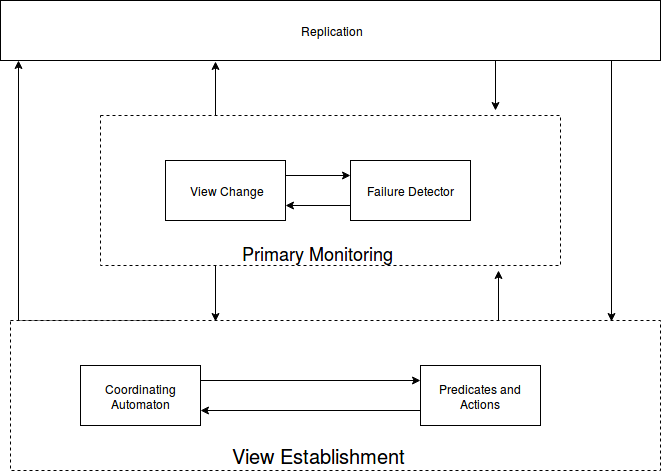
\includegraphics[scale=0.5]{ade/ssbftdiagram.png}
			        \end{center}
	           \end{figure}
	           
			\subsection{System Properties}
			    Variables \textit{N} denotes the amount of processors deployed, and the variable \textit{f} denotes the maximum amount of faulty processors that the system can have to be able to self-stabilize, and \textit{f} = (\textit{N}-1)/5. \textit{K} denotes the amount of clients sending requests to the replicas, and \textit{T} denotes a threshold timely incremented that has to exceeded in case of a non-progressive primary in order to issue a view change.
			    
			\subsection{View Establishment}
			    This module is part of the addition to Castro and Liskov's PBFT \cite{pbft} to achieve self-stabilization. It's role is to establish a consistent view and state among \textit{N-f} processors. It provides a unique view among correct processors and deploys a view change after instruction from the \textit{Primary Monitoring} module. The module is composed of two submodules, a \textit{Coordinating Automaton}, where it describes a two state automaton that establishes a lockstep transition of phases and views amid at least \textit{3f + 1} correct processors by employing a \textit{witnessing} mechanism, and \textit{View Predicates and action} which is a series of predicates and their complementary actions to describe phase and view transitions, used by the \textit{Coordinating Automaton}. The \textit{witnessing} mechanism works by exchanging messages containing the sender's current phase, view, view change flag and the receiver's last reported phase, view and view change. If the last reported phase, view and view change flag are correct to the receiver's current values, then the sender is a witness of the receiver. Upon a processor raising the view change flag and \textit{4f + 1} processors support a view change, or if \textit{4f + 1} processors issued a view change and the processor's flag is not raised ,then the next view is prepared by forwarding the next view (each processor has a current view and a next view, both starting at the same value). After preparing the next view, if the next view is establishable, then the new view is installed.
			    		

			 \subsection{Replication Module}
			    This module follows the specification of replication found in Castro and Liskov's algorithm, but with a few modifications to enable handling of stale information. In case of a consistent view among processors, the replicas progress the replication. Otherwise, a view change is requested from the \textit{View Establishment} module and retreats to a default state. As mentioned before, clients are required to send requests to all replicas, in contrast with the PBFT variation where the client sends a request only to the primary processor. This is the case because in Castro and Liskov's version requests sent to the primary by the client are cryptographically signed, so that the primary cannot tamper with the contents of the request, while in this case using cryptographically signed messages is incompatible with the property of Self-Stabilization. Thus a request is \textit{valid} if it has been seen by at least \textit{(N-f)/2+f} correct replicas. Hence, the primary still decides the order of execution of requests, but fake requests generated by the primary are handled by a self-stabilizing all-to-all communication procedure. Processors exchange their replica structure, checking whether processors have consistent, pending requests, accepted requests and replica state. While it is the primary's responsibility to assign a sequence number to a request (order it for execution), it is required that the request is seen by at least \textit{4f + 1} other processor, thus preventing the primary from assigning made-up requests for execution, or tampering with a client's request. In case of a stale replica state, a state flush is issued, and a state which is a common prefix of at least \textit{4f + 1} processors is installed.
			    		

			  \subsection{Primary Monitoring}
			    The Primary Monitoring is consisted of two sub-modules, a \textit{View Change} mechanism and a \textit{Failure Detector}. The module monitors the primary by the view change mechanism using the failure detector to decide whether or not a primary is suspected to be faulty. Failure Detector employs a heart beat mechanism, where when either the primary is not responding, the replication is not progressing or the primary is issuing invalid requests, the primary is suspected to be faulty. When at least \textit{3f + 1} correct processors suspect that the primary is fault or malicious, a view change is deployed. The failure detector is the component that exchanges heart-beat messages in the form of tokens, and keeps record of a counter and a beat for each processor. In each iteration, if a processor received a token from processor p\textsubscript{i} then \textit{beat[i]} is set to 0, otherwise \textit{beat[i]} is incremented. If the \textit{counter[i]}'s value surpasses the threshold \textit{T}, then p\textit{i} is deemed non-responding. Similarly, count[i] is incremented when processor p\textit{i} sees no progress in the replica state from the primary (i.e primary is not assigning requests for execution), thus if the counter surpasses the threshold \textit{T}, the primary is deemed to be malicious. Consequently, if a primary is suspected by the processor, and \textit{4f + 1} processors support a view change, then the view change flag is raised.
			    		

		\section{Implementation Decisions}
		    As mentioned in introduction, for the implementation of the self-stabilizing BFT algorithm I have decided to use Go as the programming language and ZeroMQ as the messaging library.
		    		

		    \subsection{Go}
		    Go's hype for being the de facto language for Networked and parallel systems is mainly the reason
		    it was selected to be the programming language of this work. Go is packaged with great parallelism tools like goroutines and channels. Goroutines are light-weight threads or green-threads, that can be instantiated simply by adding the corresponding dedicated keyword in front of a procedure call. Since for this implementation I have decided to have each module running concurrently, goroutines greatly facilitated this project's need for multi-threading support. Channels are the means to connect and synchronize concurrent goroutines. By default channels can contain only one element at a time and trying to read from an empty channel or write to a full one will send the goroutine to sleep until the operation becomes doable. Channels along with the \textit{select} statement that provides polling between multiple communication channels, is a great fit for handling inter-processor and server-client exchanges. For this project, no 3rd party libraries have been used at all, and official packages have been used to the minimum, using mostly only the most basic features of Go. 
		    		

		    \subsection{ZeroMQ}
		    ZeroMQ is a light-speed asynchronous messaging library. It provides a variety of sockets that can be used to deploy a vast amount of distributed messaging patterns in any networked topology required. ZeroMQ is state-of-the-art in terms of speed, and reliability. Unlike other messaging libraries, a ZeroMQ application can run without a dedicated messaging broker. Messages are stored in a hidden message queue making the delivery of messages guaranteed, while also being able to send a message to a node without that node necessarily being online at the time. All of these make ZeroMQ great for this application since reliability of the communication channel is important and more so the delivery of messages in order. ZeroMQ follows a simple interface that greatly facilitates usability of the library.
		    		

		    \subsection{Project Structure}
		    The project's structure is as seen in Figure \ref{fig:project_struct}. Since Go does not allow for cyclic dependencies in between packages, the files for the algorithm's modules are located in the same package, as these modules interact with each other by calling each others interface functions. In the \textit{config} folder the code for configuring the IP addresses of the system and configuring the test scenario are located. A logger is implemented that logs output and errors in text files for the monitoring of the program's operation. The \textit{types} package contains all the necessary Go \textit{structs} and type aliases required and the \textit{variables} package contains variables and constants that are shared between modules, like \textit{N} and \textit{f}. \textit{messenger} is the package responsible for sending and receiving inter-processor and client messages.
		    
		    \begin{figure}
		        \centering
		         \begin{forest}
              for tree={
                font=\ttfamily,
                grow'=0,
                child anchor=west,
                parent anchor=south,
                anchor=west,
                calign=first,
                edge path={
                  \noexpand\path [draw, \forestoption{edge}]
                  (!u.south west) +(7.5pt,0) |- node[fill,inner sep=1.25pt] {} (.child anchor)\forestoption{edge label};
                },
                before typesetting nodes={
                  if n=1
                    {insert before={[,phantom]}}
                    {}
                },
                fit=band,
                before computing xy={l=15pt},
              }
                [SSBFT
                  [app
                    [messenger
                        [messenger.go]]
                    [coordination.go]
                    [establishment.go]
                    [faildetect.go]
                    [replication.go]
                    [viewchange.go]
                  ]
                  [config
                    [local.go]
                    [planetlab.go]
                    [scenario.go]
                  ]
                  [logger
                    [logger.go]
                  ]
                  [types
                    [clientmessage.go]
                    [coordination.go]
                    [request.go]
                    [...]
                  ]
                  [variables
                    [variables.gop]
                  ]
                  [main.go]
                ]
              \end{forest}
    		        \caption{Project Structure}
    		        \label{fig:project_struct}
    	    \end{figure}{}
    	    		

		    \subsection{Processor}
		    Processors send and receive messages between other processors and their clients through concurrent goroutines. After the initialization of the program, a go-routine is launched for each of the algorithm's modules and for the messenger component (see Figure \ref{fig:main_go}. Replication modules of each processor exchange in an all-to-all manner their current replica state. In the same manner \textit{Coordination} components exchange coordination info, \textit{fault detectors} exchange tokens containing information about primary suspicion and acting as a heartbeat, and the \textit{View Change monitors}  exchange information about changing views. For each type of inter-processor message there is a Go channel in the \textit{messenger} component that asynchronously write incoming messages in, and the corresponding module asynchronously consumes said message and takes the appropriate action. For instance, there is a channel for replica states, a channel for coordination messages and so on. When receiving a client request, it is added to the pending requests queue (again through the use of a channel), and after being assigned a sequence number from the primary, and executed by all processors, the replica state is sent back to the client. For this example, the replica states is consisted of an array of characters, and the available operations that a client can request are only 'ADD', since it is out of the scope of this work to examine the possible applications of this algorithm.
		    
		    \subsection{Client}
		    Similarly, the client program is implemented in go and has a similar project structure like that of the server's program consisted of \textit{config, logger, messenger} and \textit{variables}. The client sends a request that contains a character and an operation, to all of the replicas and awaits for \textit{f + 1} identical responses before moving on to the next request. In the context of this project, the system interacts with only one client, since it is not in the scope of this work the investigation of how many clients such a system can support.
		    
		    		

		\section{Implementation Description}
		       \begin{figure}
		        \centering
		         \begin{lstlisting} 
                    package main
        
                    ...
                    func main() {
            
                        ...
                        go messenger.TransmitMessages()
                    	go app.FailDetector()
            	        go app.ByzantineReplication()
        	            go app.ViewChangeMonitor()
        	            go app.CoordinatingAutomaton()
                    }
                 \end{lstlisting}
		        \caption{Launching Goroutines for each Module}
		        \label{fig:main_go}
		    \end{figure}
		    At the beginning of the program, and after all the initializations are done, a goroutine is launched for each of the modules as shown in Figure \ref{fig:main_go}. Each module operates concurrently with each other and exchange information by calling each other's interface functions. Also goroutines are launched for sending and receiving messages, synchronizing the process by the use of channels, so that the execution of a program behaves like a its components are independed (see \ref{fig:thread_arch}.
		    
		    \begin{figure}
		        \centering
		        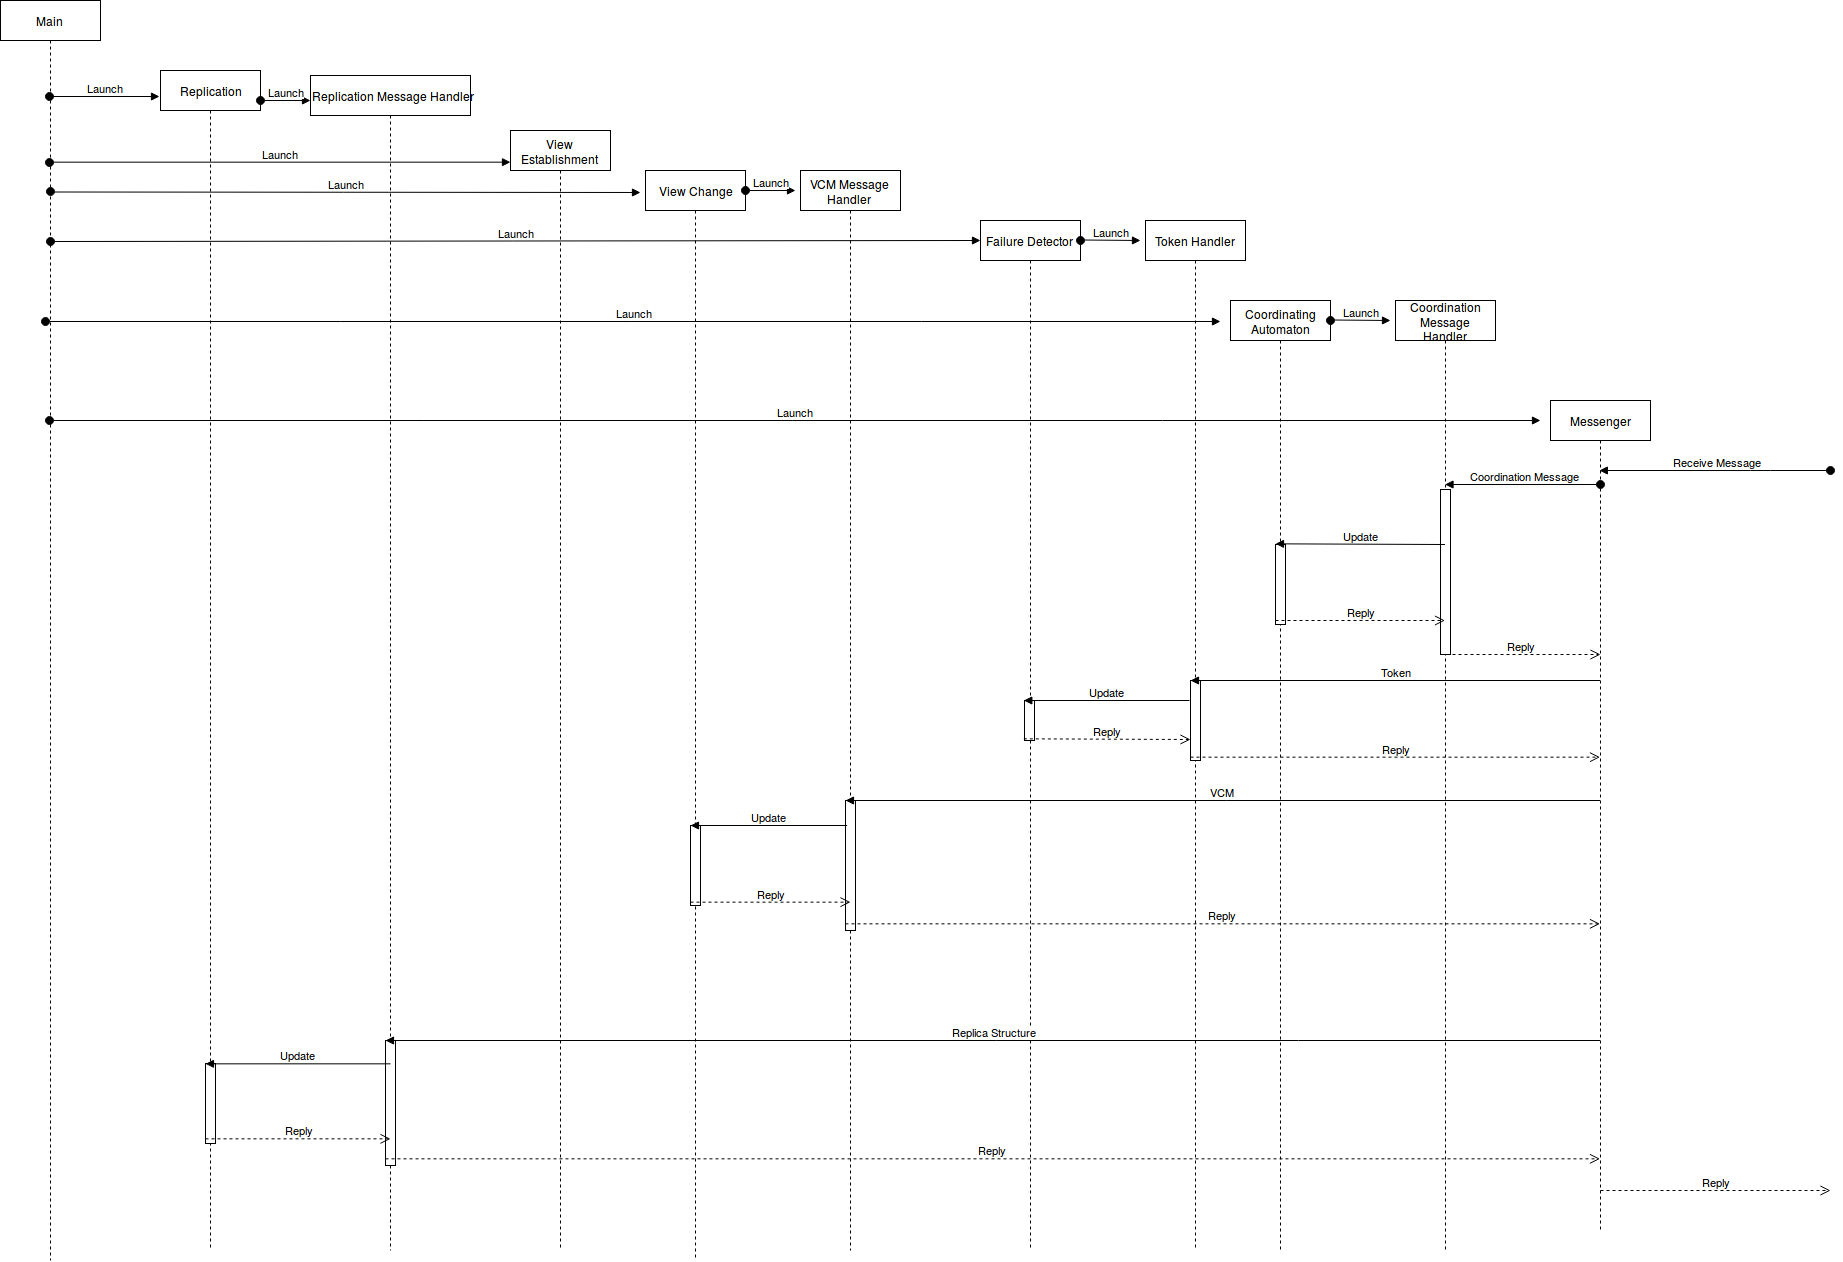
\includegraphics[scale = 0.25]{ade/thread_architecture.png}
		        \caption{Thread Architecture Sequence Diagram}
		        \label{fig:thread_arch}
		    \end{figure}
	     
		    \begin{figure}
		        \centering
		         \begin{lstlisting}
                   func (vcm *VCM) GobEncode() ([]byte, error) {
                    	w := new(bytes.Buffer)
                    	encoder := gob.NewEncoder(w)
                    	err := encoder.Encode(vcm.VStatus)
                    	if err != nil {
                    		logger.ErrLogger.Fatal(err)
                    	}
                    	err = encoder.Encode(vcm.Prim)
                    	if err != nil {
                    		logger.ErrLogger.Fatal(err)
                    	}
                    	err = encoder.Encode(vcm.NeedChange)
                    	if err != nil {
                    		logger.ErrLogger.Fatal(err)
                    	}
                    	err = encoder.Encode(vcm.NeedChgSet)
                    	return w.Bytes(), nil
                    }
                 \end{lstlisting}
		        \caption{Example implementing GobEncoder}
		        \label{fig:encoder}
		    \end{figure}
		   \subsection{Sending data structures and Gob}
		   \begin{figure}
		        \centering
		         \begin{lstlisting} 
                    func (vcm *VCM) GobDecode(buf []byte) error {
                    	r := bytes.NewBuffer(buf)
                    	decoder := gob.NewDecoder(r)
                    	err := decoder.Decode(&vcm.VStatus)
                    	if err != nil {
                    		logger.ErrLogger.Fatal(err)
                    	}
                    	err = decoder.Decode(&vcm.Prim)
                    	if err != nil {
                    		logger.ErrLogger.Fatal(err)
                    	}
                    	err = decoder.Decode(&vcm.NeedChange)
                    	if err != nil {
                    		logger.ErrLogger.Fatal(err)
                    	}
                    	err = decoder.Decode(&vcm.NeedChgSet)
                    	if err != nil {
                    		logger.ErrLogger.Fatal(err)
                    	}
                    	return nil
                    }
                 \end{lstlisting}
		        \caption{Example implementing GobDecoder}
		        \label{fig:decoder}
		    \end{figure}
		   Since most of the messages that are exchanged in the system are complex structures containing multiple fields, some of which could also be complex structures, and ZeroMQ sends messages as a sequence of bytes, a method of serialization and deserialization of structs is necessary. For this requirement we used Gob\cite{gob}. Gob is a package included in Go's standard library, and it manages streams of bytes exchanged between an Encoder (usually the transmitter) and a Decoder (usually the receiver). Encoding with Gob returns an array of bytes while decoding with Gob builds a struct from an array of bytes
		   
		   Gob supports encoding and decoding of all Go's built-in types, but to be able to encode/decode a complex struct, that struct has to implement the GobEncoder/GobDecoder interface by implementing GobEncode/GobDecode methods (as seen in Figures \ref{fig:encoder} and \ref{fig:decoder}). Fields of a struct that are also structs have to also implement the GobEncoder/GobDecoder interfaces. Only exported fields of a struct can be encoded/decoded using Gob, so exchanged structs are required to have all their fields public.
		    
		     		

		    \subsection{Messenger}
		        \paragraph{First Approach}
    		    The \textit{messenger} component might have been the hardest part to implement. Implementation of this component has gone through numerous iterations. First attempt was to have in each processor a pair of ZeroMQ's PUB/SUB sockets for publishing and receiving updates from and to the rest of the processors, and another pair of PUB/SUB sockets for subscribing to requests from clients and replying through publishing (as shown in Figure \ref{fig:pubsub}). This had a number of issues. Mainly processors and clients had to know where did the message come from. That was easily solvable by including another field in the body of the message indicating the identity of the sender. Other than that, messages exchanged through PUB/SUB sockets are not persistent, meaning that if a receiver is disconnected at the time for some reason, then any messages sent to it are lost. So that means that any messages sent before some processor/client was instantiated are lost.
    		     \begin{figure}
    		        \centering
    		        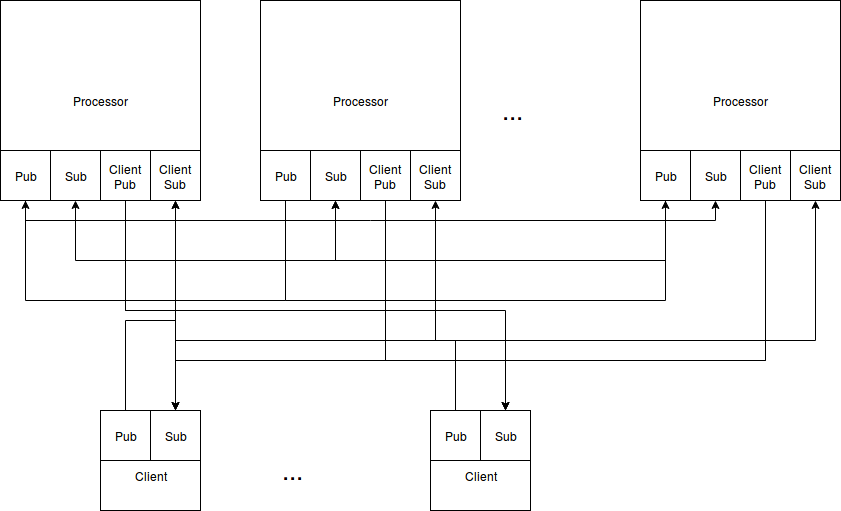
\includegraphics[scale = 0.4]{ade/messenger1.png}
    		        \caption{First Messaging Pattern attempt.}
    		        \label{fig:pubsub}
    		    \end{figure}
    		    		

    		    \paragraph{Second Approach}
    		    A second approach (shown in Figure \ref{fig:syncedpubsub}) was deploying a synchronized PUB/SUB architecture. It would require an extra pair of REQ/REP sockets in each processor, of which messages are persistent, to exchange an "Online" message so that processors would start exchanging messages only if all processors are instantiated. But even then, PUB/SUB sockets are not reliable in the meaning that there's no message queue under their implementation, thus if the receiver could not keep up with the incoming messages then some messages would be dropped (Although sending infinitely many messages means receiving infinitely many, so that could possibly be feasible).
    		   		

    		    \paragraph{Third Approach}
    		    A latter approach was trying to use solely REQ/REP pairs of sockets. This way, messages were guaranteed to reach their destination in order. To implement such a pattern, each processor needs to have a REQ/REP socket for each other processor and client. However, from the specification of the algorithm, processors in each cycle of \textit{Replication} module send back to the clients the last executed request, even if the client has already received a reply and hasn't sent another request. This conflicts with the mandatory send, receive, send, receive and receive, send, receive, send operation sequences of REQ and REP sockets.
    		     \begin{figure}
    		        \centering
    		        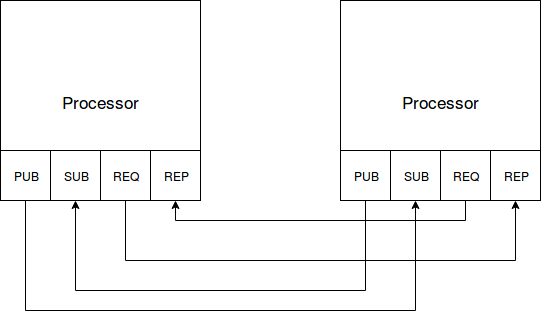
\includegraphics[scale=0.6]{ade/messenger2.png}
    		        \caption{Overview of Synchronized PUB/SUB pattern}
    		        \label{fig:syncedpubsub}
    		    \end{figure}
    		    		

    		    \paragraph{Final Solution}
    		    The eventual solution was a modification of our third approach, where each processor has a REQ/REP pair of socket for each other processor and client, while adding an extra PUB socket for each client, and clients deploy a REQ/REP pair along with an extra SUB socket for each processor (as shown in \ref{fig:finalmessenger}. This way processors intercommunicate with the use of their corresponding pair, while clients send requests to processors through a REQ/REP pair, only now the processor will immediately reply with an empty message, rendering it's REP socket available for the next request, and requests' results are being sent through the publisher socket until the client replies with an ACK message. With this solution, there won't be cases where REP sockets try to receive twice consecutively, or REQ sockets tyring to send twice, an error which would otherwise cause an error and crash the system. Processors will keep sending to the client the last client's executed request result until a client responds with 'ACK', something that happens only when the client has received \textit{f+1} identical response results, suggesting correct execution of the algorithm.
    		    
    		    \begin{figure}
    		        \centering
    		        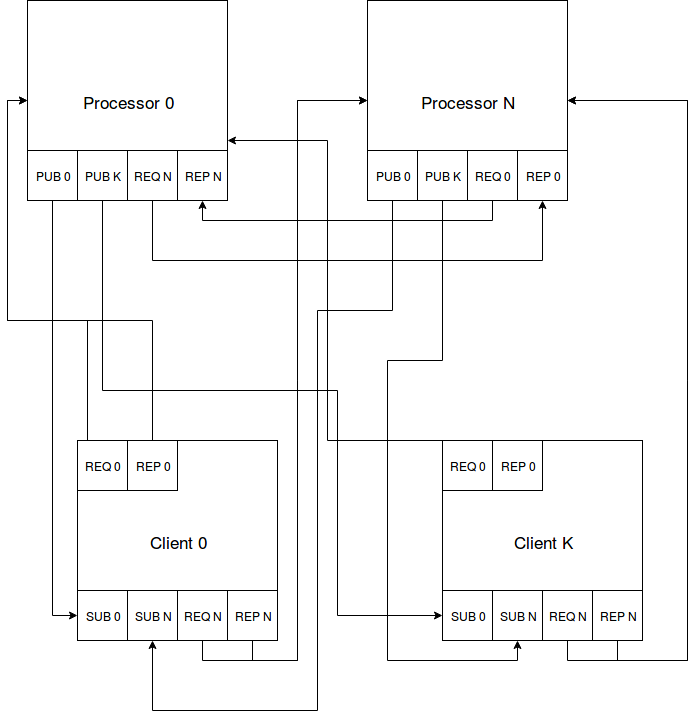
\includegraphics[scale = 0.5]{ade/finalmessenger.png}
    		        \caption{Final solution for Communication}
    		        \label{fig:finalmessenger}
    		    \end{figure}
    		    		

	        \subsection{Passing Messages to corresponding modules}
	            Processors' messages are wrapped in a structure that is composed of the fields \textit{Payload}, which is an array of bytes, a string \textit{Type} that denotes the type of the payload in terms of the name of the structure, and an integer \textit{From} denoting the identity of the sender processor. When the messenger component receives an incoming message, it decodes received bytes into a \textit{Message} struct, and then a switch case is applied on the structure's \textit{Type} field. The message's payload is the decoded as well to the appropriate struct type, and the resulting struct is consequently written to the corresponding channel, in which of the consumer module will read from. This pattern succeeds on hiding delays of sending and receiving messages, making the message exchange feel more organic. Furthermore all code for handling and sending messages are also launched in separate goroutines.
	            \begin{figure}
	                \centering
	                \begin{lstlisting}
	                   type Message struct {
                        	Payload []byte
                        	Type    string
                        	From    int
                        }
	                \end{lstlisting}
	                \caption{Message wrapper struct}
	                \label{fig:messagestruct}
	            \end{figure}
	            		

	        \subsection{Mapping IP addresses to nodes}
	            For local development, the mapping of network addresses to nodes happen in the \textit{local.go} file. It contains four maps of strings to integers, each map storing the corresponding address of the appropriate socket type. For developing and running locally, the code is found in Figure \ref{fig:ipconfiguration}, where \textit{MapOfAddresses[address]==i} represents the address of the corresponding socket of processor p\textsubscript{i}. Similarly, for the PlanetLab configuration, instead of tinkering with ports, each processor has it's own computer and IP address (see \ref{fig:ipconfigglobal}
	            
                \begin{figure}
                \centering
                \begin{lstlisting}
var RepAddresses map[string]int
var ReqAddresses map[string]int
var ServerAddresses map[string]int
var ResponseAddresses map[string]int

func InitialiseIP(n int) {
	RepAddresses = make(map[string]int, n)
	ReqAddresses = make(map[string]int, n)
	ServerAddresses = make(map[string]int,
	        variables.K)
	ResponseAddresses = make(map[string]int,
	    variables.K)
	for I := 0; I < n; i++ {
		RepAddresses["tcp://localhost:"+
		    strconv.Itoa(
		        4000+variables.Id*100+i
		    )] = i
		ReqAddresses["tcp://localhost:"+
		    strconv.Itoa(
		        4000+i*100+variables.Id
		    )] = i
	}
	for I := 0; I < variables.K; i++ {
		ServerAddresses["tcp://*:"+
		    strconv.Itoa(7000+variables.Id*100+i)] = i
		ResponseAddresses["tcp://*:"+
		    strconv.Itoa(10000+variables.Id*100+i)] = i
	}
}
                \end{lstlisting}
                \caption{IP configuration for local execution}
                \label{fig:ipconfiguration}
                \end{figure}
                
                \begin{figure}
                    \centering
                        \begin{lstlisting}
var RepAddressesIp map[string]int
var ReqAddressesIp map[string]int
var ServerAddressesIp map[string]int
var ResponseAddressesIp map[string]int

func InitialiseIp(n int) {
	RepAddressesIp = make(map[string]int, n)
	ReqAddressesIp = make(map[string]int, n)
	ServerAddressesIp = make(map[string]int, variables.K)
	ResponseAddressesIp = make(map[string]int, variables.K)
	for i := 0; i < n; i++ {
		RepAddressesIp["tcp://*:"+
		        strconv.Itoa(4000+i)] = i
		ReqAddressesIp["tcp://"+
		        addresses[i]+":"+
		        strconv.Itoa(4000+i)] = i
	}
	for i := 0; i < variables.K; i++ {
		ServerAddressesIp["tcp://*:"+
		    strconv.Itoa(7000+variables.Id*100+i)] = i
		ResponseAddressesIp["tcp://*:"+
		    strconv.Itoa(10000+variables.Id*100+i)] = i
	}
}
                        \end{lstlisting}
                    \caption{IP configuration for PlanetLab execution}
                    \label{fig:ipconfigglobal}
                \end{figure}
	            
    		    
		   
	\newpage
	\chapter{Experimental Assessment}
	    For the experimental assessment of the algorithm, the experiments are going to be executed over at PlanetLab Europe\cite{planetLab} to really acquire an idea how would the self-stabilizing BFT would cope in a real-world like simulation. Experiments done are a series of scenarios, some of them having faults seeded in the program, that the algorithm should handle and cope with, eventually self-stabilizing and continuing its regular operation.
		\section{PlanetLab}
		PlanetLab \cite{planetLab}, founded in 2002, is a global computer network available as a test platform for computer networking and distributed systems research. Since December 2011, PlanetLab has 1,024 nodes in 530 locations worldwide. Each research program performs a "slice" that gives access to the experimenters to a virtual machine on each node associated with that piece.
% 		For more details, please refer to the PLE statistics page.
		Universities and corporations provide nodes to PlanetLab in return for accounts for the use of the network. PlanetLab is a planetary-wide network, making this the perfect environment for evaluating the performance and behavior of this paper's project.
		
		\section{Experiment Scenarios}
    		The experiments is a series of scenarios, some of them having faults injected in the system, constructed with the intention of evaluating the following: 
    		\begin{itemize}
                \item The correctness of the algorithm operating under a legal state.
    			\item The ability of self-stabilizing in various scenarios where processors are faulty.
    			\item The performance of the system when trying to self-stabilize and the cost of self-stabilizing.
    			\item The overhead cost of self-stabilization in comparison with a classical BFT implementation
    		\end{itemize}
    		
    		\subsection{Normal Operation}
    		The first experimental scenario is running the system over at PlanetLab with a legal initial state evaluating the correctness of the algorithm under legitimate operation  and measuring the average request execution time, the average service time and the average number of messages exchanged and comparing the measurements with the execution of the same system but having the modules needed for self-stabilization disabled. Thus having a close correlation of the self-stabilizing BFT by Dolev et al. and the classical version of BFT by Castro and Liskov.
    		
    		\subsection{Stale Views}
    		Subsequently, the next scenario launching the system by having an illegal initial state with \textit{f - 1} processors having a different view. This is done by having an if statement in the initialization where in processor\textsubscript{i} if \textit{i\%(N/F)==0} we set the local primary to 1 (instead of 0 which is the default initial primary). In this scenario, processors have to acknowledge that the view is not consistent among them and a new view should be issued afterwards. Average time of issuing a new view is measured here.
    		
    		\subsection{Stale States}
    		Similarly as in the Stale Views scenario, in this scenario the system is bootstrapped with an illegal initial state with \textit{f - 1} processors having stale states. In essence, faulty processors will be initialized with a non-empty Replica State. Here, by exchanging replicas in the \textit{Replication} module, processors should be able to notice the inconsistency between replicas' states, and a new state should be issued. Along with the usual measurements, time of converging into a consistent replica state is also measured.
    		
    	    \subsection{Primary Byzantine}
    	    This scenario assesses the Byzantine Fault Tolerance part of the algorithm. Having the initial primary processor being malicious, the system should proceed to the next view. This scenario is actually consisted of three sub-scenarios, having a primary processor which isn't responding at all, having a primary processor which issues made-up requests for execution and a primary which sends false information to the rest of the processors.
    		
    		
		\section{Experiment Results}
		After running the aforementioned experiments over at the PlanetLab, we got some rather interesting results. 
% 		Unfortunately the system we built, could not self-stabilize in the cases of having a byzantine primary. So our measurements in that department might not be correct. When having a malicious primary, our system would fall into some kind of a deadlock where a View Change will be requested and the next view will be set by the Coordinating automaton, but after that, the \textit{AllowService} interface function which allows nodes to proceed with their operation under some conditions, would always return \textit{false},  thus resetting the failure detector and as follows the primary would no longer be \textit{"suspected"}, before being able to establish the new view.
		
		\begin{figure}
		    \centering
		    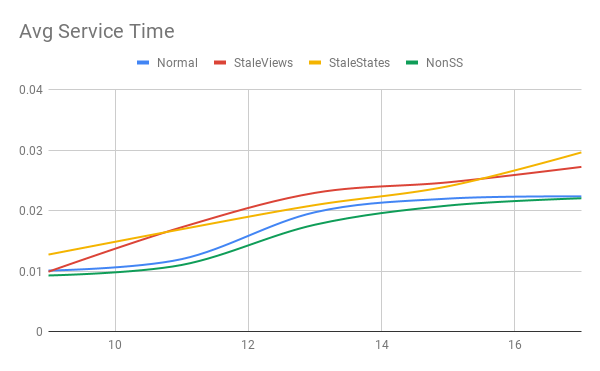
\includegraphics[scale = 0.7]{ade/AvgServiceTime.png}
		    \caption{Average Service Time}
		    \label{fig:servicetime}
		\end{figure}
		
		 We can observe that the overhead for seventeen server processors is only 8\%, and from the graph we can deduce that the overhead is decreasing as nodes increase. We can also see that, in general, as nodes are increasing, the average service time converges to some extent.
		The reason of having an increased average service time as nodes increase, probably lies in the fact that as processors increase, so do the exchange of messages between them.
		
		We can also notice that converging from a stale state, is faster than converging from a stale view for low number of nodes, but for larger values, the average service time of the stale view scenario is stabilizing while the stale states scenario keeps increasing. Obviously the more requests that are processed, the closer the curves between the faulty scenarios and the ordinary one will be.
		
		\begin{figure}
		    \centering
		    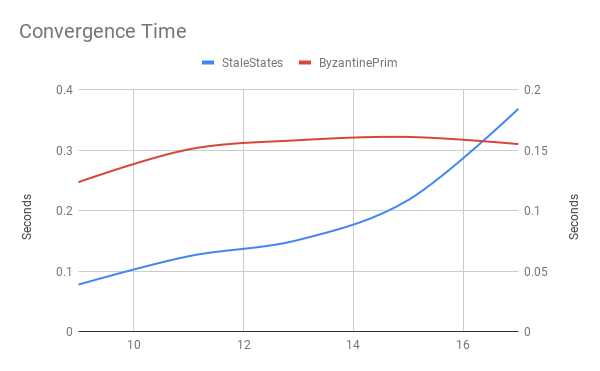
\includegraphics[scale=0.7]{ade/Convergence_Time.png}
		    \caption{Average Convergence Time}
		    \label{fig:convergencetime}
		\end{figure}
		
% 		While we cannot guess what is the average convergence time in the scenario of the malicious primary processor, we can still look for a lower bound, since the system \textbf{did} recognize the malicious primary \textit{and} prepared the next state before deadlocking.
		From the Chart \ref{fig:convergencetime} we can see that the time that it takes to detect a malicious primary and prepare the next view is roughly ten times that of the time required to serve a request. While restoring from a stale state is roughly equal to five times the average service time of a request. We also note that the time for self-stabilizing from a byzantine primary is stable, in contrast with the convergence time from a stale state. This probably stems from the fact that the overhead of requiring additional nodes to suspect a malicious primary is not as relevant as the overhead that is produced by the increased amount of messages exchanged in the case of a stale state.
		
		\begin{figure}
		    \centering
		    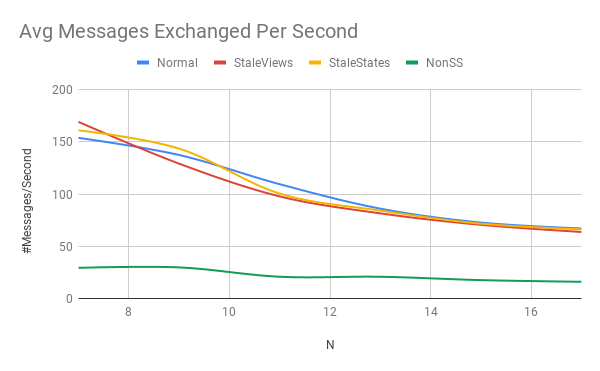
\includegraphics[scale=0.7]{ade/avgexchange.png}
		    \caption{Average Messages Exchanged Per Second}
		    \label{fig:avgmsg}
		\end{figure}
		
		Finally, observing the chart \ref{fig:avgmsg}, we notice that the average amount of messages exchanged by processors is approximately 6 times larger in the self-stabilizing version of the system than that of it's analogous non self-stabilizing, even though this overhead is not seen in the service time. This is probably because of the fact that the self-stabilizing version utilizes parallelism better in the form of threads. The non-self-stabilizing version is the same system but just having disabled the go-routines that launch the modules necessary only for self-stabilization. Also the amount of messages exchanged in the correct scenario is roughly the same as the scenario's with faulty illegal state, which was expected.
	
		\section{Summary}
	 We concluded that the overhead of the self-stabilizing version of our system is roughly 8\%, and that the cost of self-stabilizing from an illegal state is more or less seven times the time that the system requires to serve a request, and the convergence time from a byzantine primary is about ten times that of the average service time.
	\newpage
	\chapter{Conclusions}
		\section{Summary}
		After researching the literature about Distributed Systems and Self-Stabilization, we've decided that the best fit for the purpose was using the Go programming language along with ZeroMQ library as the messaging channel. We designed a set of experiments with the goal of testing the capabilities of the algorithm and our implementation in terms of performance and the ability to self-stabilize. Unfortunately, our implementation did not succeed to self-stabilize in the experiment where the system was initialized with a faulty primary, though we acquired some rather valuable results. We achieved an 8\% overhead compared to the non-self-stabilizing version of our system, and the cost of self-stabilizing from an illegal state being roughly seven times the time required for the system to serve a request, and for self-stabilizing from a malicious primary is approximately ten times the average serve time.

		\section{Notable Difficulties}
		Most difficult part of this project was building the inter-processor communication, as it took us a number of iterations before reaching to an acceptable implementation, along with the serialization and deserialization of complex structs to a series of bytes, since the API of ZeroMQ supports only the delivery of bytes. Also a great difficulty appeared to be the debugging of the system, since debugging a distributed system is much more challenging than debugging a single processor program, let alone debugging a distributed system with multi-threading. Other difficulties were translating the algorithm from a formal language to the Go programming language, since Go doesn't quite support functional programming and it's a quite verbose language (the code for the processor application reached over 3.5 thousand lines), and the design of the system in terms of types, components etc. Lastly, I've encountered a number of faults in the description of the algorithm (e.g structure types were inconsistent at points) and a lot of corrections were done in the process, consequently validating the description of algorithm at the same time.
		\section{Retrospection}
		As mentioned in in Subsection 3.2.3, all of our components were located in the same package. That means that non-exported variables, functions and methods were still shared between them. Although for the purpose of this research this did not affect our implementation by any means, a decoupled package communication approach could be followed where modules/packages communicate with each other through the use of a bus package. Our decision to avoid 3rd party libraries has also hindered the development as a lot of tedious code had to be written (for instance slice and list helpers that provide methods like \textit{AppendIfMissing} since they are not provided by default), and Go is a very verbose programming language. Lastly, although Go is a very good language (and a favorite of mine) and it has facilitated the development of a distributed multi-threaded system by a lot, using an object oriented language with better support for functional programming, like Java or Scala, would help minimize the size of the code base by a lot.
	\newpage

	\bibliographystyle{plain}
	\bibliography{sources}

\end{document}
